\documentclass[12pt]{article}
\usepackage{graphicx}
\usepackage{subcaption}
\setlength{\parindent}{0pt}
\setlength{\parskip}{10pt} % block paragraphs
\usepackage{bm}
\begin{document}

\title*{\centerline{\LARGE{CAP 5619 \-- Deep and Reinforcement Learning}}}
\author*{\centerline{Project2 Hua Huang}}%unnumbered centered head

\section{Task I-Recurrent Neural Network Design}
A LSTM RNN is used in this project, 2 LSTM layers are used here and
each layer has 100 hidden units. The loss function is categorical
crossentropy here, and learning rate is 0.005.

\section{Language Models for Protein Sequences and Evaluation}
The kernel is initialized as 
$TruncatedNormal(mean=0.0, stddev=0.1)$, the biases are
initialized as $Constant(value=0.5)$.\\
The optimizer is $Adam(lr=0.005, beta_1=0.9, beta_2=0.999,
epsilon=None, decay=0.0, amsgrad=False)$, which is the most popular
one in the deep learning community currently. The training history is 
recored in Fig.1 and Fig.2.\\
\begin{figure}[h]
    \centering
    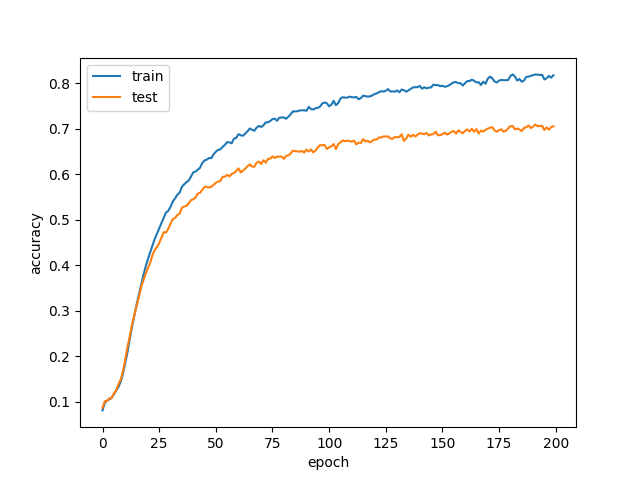
\includegraphics [scale=0.5]{accuracy.png}
    \caption {Training history of accuracy}
\end{figure}

\begin{figure}[h]
    \centering
    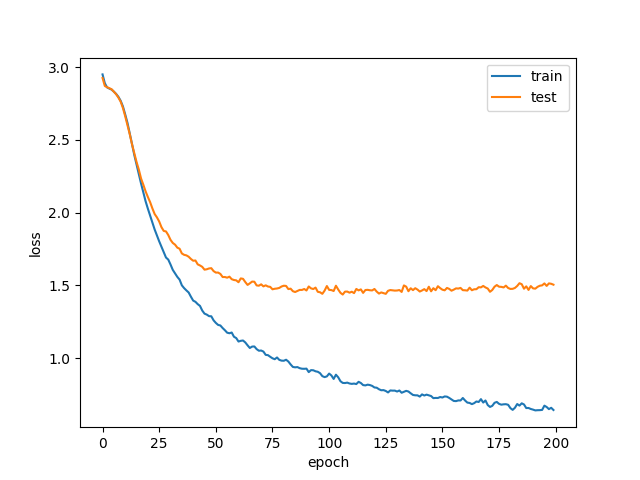
\includegraphics [scale=0.5]{loss.png}
    \caption {Training history of loss}
\end{figure}
To have an intuitive understanding of the capturing of the long\--term
dependence, an experiment is carried here, in which the input sequence
is based on the 1st sample in the test set. The 1st char is changed
from \textit{K} to \textit{L}. Correspondingly, the output sequences are
\begin{eqnarray}
    \scriptstyle{KLSEGEWQLVLHVWAKVEADVA\bm{G}HGQDILIRLFKSHPETLEKFDRFKHLK} \\ \nonumber
    \scriptstyle{LYVPSHKYISNIFTHKFTVHKQ\bm{G}HGFLILIRLLKSHPDTLPKLDRFRHLK} \nonumber
\end{eqnarray}
We can see after 22 chars and begin with $G$ there is no consecutive chars 
in the new sequence that are different from the old sequence, we can say the 
memory is about length of 22. 

\subsection{Sequence Generation Techniques}
To demonstrate the generation techiniques, 8 sequences chosen from the
test samples are used as materials. The first 10 chars for each
sequence are kept, and the model is asked to generate the next 10 chars.
Then the original sequences are compared with the generated sequences.
The model is supposed to be able to generate similar sequences
compared with the original one, and the results are:\\
sample 1:\\
MVLSEGEWQL VLHVWAKVEA\\
MVLSEGEWQL VLHVWAKVEA\\

sample 2:\\
STAGKVIKCK AAVLWEEKKP\\
STAGKVIKCK AAVLWEEKKP\\

sample 3:\\
ETELAFLYER DIYRLLAECD\\
ETELAFLYER DIYRLLALQA\\

sample 4:\\
MTEPLILQPA KPADACVIWL\\
MTEPLILQPA KPADAVAPDK\\

sample 5:\\
VQAVAVLKGD AGVSGVVKFE\\
VQAVAVLKGD AGVSGHASIQ\\

sample 6:\\
MSKGEELFTG VVPILVELDG\\
MSKGEELFTG HTPPIDGVGK\\

sample 7:\\
VTSYTLSDVV SLKDVVPEWV\\
VTSYTLSDVV SLKDVVATCK\\

sample 8:\\
MENLNMDLLY MAAAVMMGLA\\
MENLNMDLLY MAAAVMMGLA\\
We can see based on the preceding 10 chars, we can guess the next
10 chars reasonabbly well. In summary, the generation is successful.\\

The table is given in Tab1. In which, the maximum match is measured as
how many chars match with the original sequence exactly after the
leading $k$ seed input. For example, after $k$, the follow $m$ chars are
exactly the same with the corresponding chars at the original
sequences, but the $m+1$ char is different than the $m+1$ char in the
original sequence, then the match number will be $m$.
\begin{table}[h]
    \footnotesize
    \caption{Num of sequences with the given maximum mathches}
    \centering
    \begin{tabular}{*{21}{c}}
        \hline\hline
        k  & 0  & 1   &2   &3   &4   &5   &6   &7   &8   &9   &10  &11  &12  &13  &14  &15  &16 &17  &18 &19+\\
        \hline
        1  &679 & 89 & 26  &2   &9   &3   &0   &5   &2   &0   &0   &1   &1   &1   &0   &0   &0   &0  &0   &62  \\
        2  &506 & 68 & 8   &14  &4   &3   &7   &9   &3   &2   &5   &3   &4   &3   &1   &1   &1   &3  &4   &231 \\
        3  &267 & 37 & 27  &18  &9   &27  &20  &12  &14  &12  &10  &9   &9   &6   &7   &9   &12  &13 &9   &353 \\
        4  &172 & 48 & 23  &12  &40  &26  &19  &20  &13  &12  &11  &13  &11  &8   &11  &13  &15  &10 &6   &397 \\
        5  &173 & 34 & 13  &47  &32  &23  &22  &14  &13  &12  &16  &12  &8   &11  &14  &15  &10  &6  &6   &399 \\
        6  &157 & 35 & 57  &36  &27  &23  &14  &14  &12  &16  &13  &10  &12  &14  &15  &10  &6   &6  &9   &394 \\
        7  &153 & 75 & 39  &29  &26  &14  &16  &16  &16  &15  &12  &13  &14  &15  &10  &6   &6   &9  &10  &386 \\
        8  &202 & 54 & 32  &28  &17  &16  &17  &16  &15  &12  &13  &14  &15  &10  &6   &6   &9   &10 &11  &377 \\
        9  &200 & 47 & 43  &21  &18  &22  &17  &17  &14  &13  &14  &15  &11  &7   &7   &9   &10  &11 &2   &382 \\
        10 &197 & 66 & 31  &21  &24  &17  &18  &16  &14  &14  &16  &11  &7   &7   &10  &10  &11  &2  &10  &378 \\
        11 &212 & 63 & 30  &27  &19  &19  &16  &14  &15  &18  &11  &7   &7   &10  &10  &11  &2   &10 &13  &366 \\
        12 &205 & 65 & 33  &23  &26  &20  &16  &16  &20  &14  &7   &7   &10  &10  &11  &2   &10  &14 &11  &360 \\
        13 &226 & 55 & 29  &31  &21  &19  &17  &22  &14  &7   &8   &11  &10  &11  &3   &10  &14  &11 &7   &354 \\
        14 &214 & 66 & 42  &29  &20  &18  &22  &17  &7   &8   &11  &10  &12  &3   &10  &14  &11  &8  &4   &354 \\
        15 &224 & 74 & 35  &28  &19  &25  &19  &8   &9   &11  &10  &12  &3   &10  &14  &11  &8   &4  &7   &349 \\
        16 &233 & 68 & 38  &23  &33  &20  &8   &10  &12  &11  &13  &3   &11  &14  &11  &8   &4   &7  &5   &348 \\
        17 &241 & 60 & 34  &40  &26  &11  &11  &13  &11  &13  &5   &12  &14  &12  &9   &4   &8   &5  &6   &345 \\
        18 &246 & 66 & 49  &30  &13  &12  &15  &12  &13  &5   &12  &14  &12  &9   &6   &8   &5   &6  &17  &330 \\
        19 &240 & 89 & 41  &21  &13  &15  &13  &13  &5   &12  &15  &12  &9   &6   &8   &7   &6   &17 &7   &331 \\
        \hline\hline
    \end{tabular}
\end{table}

\end{document}


